\begin{multicols*}{2}
\section*{3. Функция Эйлера.\\Число красных дробей}
{\large
Пусть у нас имеется натуральное число $n$. Рассмотрим все натуральные числа, не превосходящие $n$, и выберем из них те, которые взаимно просты с числом $n$. Количество этих чисел обозначим через $\phi(n)$.

Например, для $n=8$ такими числами будут 1, 3, 5,7, и тем самым $\phi(8)=4$.

Итак, каждому натуральному числу $n$ сопоставлено число $\phi(n)$. Это соответствие $\phi$ называется \textit{функцией Эйлера}.

Перечислим некоторые свойства функции Эйлера:\\
1) $\phi(n) < n$.\\
2) Если $n = p$ - простое число, то $\phi(p) = p - 1$.\\
3) Для $n > 2$ число $\phi(n)$ четно.\\
4) Если $n = p^d$ - степень простого числа $p$, то
\[
\phi(p^\alpha) = p^\alpha - p^{\alpha-1} = p^\alpha\left(1 - \frac{1}{p}\right)
\]
5*) Если $m$ и $n$ взаимно просты, то\\ $\phi(mn) = \phi(m)*\phi(n)$\\
6) Общая формула для $\phi(n)$ такова:
\[
\phi(n) = n\left(1 - \frac{1}{p_1}\right)\left(1 - \frac{1}{p_2}\right)\dots\left(1 - \frac{1}{p_r}\right);
\]
здесь $p_1, p_2, \dots, p_r$ - все простые числа, на которые делится $n$. (Эта формула доказана в статье <<Малая теорема Ферма>>, <<Квант>>, 1972, № 10.)

Доказать все эти свойства мы предлагаем читателю. Объясним только свойство 3). Все числа, меньше, чем $n$ и взаимно простые с $n$, можно разбить на все пары: каждая пара состоит из таких чисел $q, s$, что $q+s=n$. Таким образом, число $\phi(n)$ - четно.

Число \texttt{красных} дробей в $n$-й строчке $F_n$, очевидно, равно $\phi(n)$, так как несократимых дробей $m/n\quad (0\le m/n\le 1)$ со знаменателем $n$ столько же, сколько натуральных чисел $m$, меньших, чем $n$, и взаимно простых с $n$.

Вопрос о том, сколько всего членов содержит $n$-й ряд Фарея $F_n$, обсуждает в своем письме читатель <<Кванта>> \texttt{А. Китаев} из Ленинграда.\columnbreak
\begin{center}
\begin{tabular}{|c|cccccccccc|}
\hline
$n$&1&2&3&4&5&6&7&7&9&...\\
\hline
$\phi(n)$&1&1&2&2&4&2&6&4&6&...\\
\hline
$\Phi(n)$&2&3&5&7&11&13&19&23&29&...\\
\hline
\end{tabular}
\end{center}
\caption{Таблица 2. Функция Эйлера и число дробей $F_n$}\\\\Ясно, что это число - обозначим его $\Phi(n)$ - равно\\
$\Phi(n) = 1+\phi(1)+\phi(2)+\phi(3)+\dots+\phi(n)$,\\поскольку $\Phi(1) = 2$ и $\Phi(n) = \Phi(n-1)+\phi(n)$ (см. таблицу 2). Простой формулы для $\Phi(n)$, видимо, не существует. Но интересно, что, несмотря на крайне нерегулярное поведение функции Эйлера $\phi(n)$ (отношение $\displaystyle\frac{\phi(n)}{n}$ бывает сколь угодно близко и к 0, и к 1), для $\Phi(n)$ можно доказать такое предельное отношение:
\[
\lim_{n \to \infty}\frac{\Phi(n)}{n^2} = \frac{3}{\pi^2} \approx 0{,}305\dots,
\]
т.е. $\Phi(x)$ при больших $x$ возрастает <<приблизительно по параболе>>: $\displaystyle \Phi(x) \approx \frac{3}{\pi^2}x^2$

Это - одна и красивых теорем, полученных австрийским математиком Ф. Мертенсом (1874 г.).
}
\section*{4. Соседние знаменатели}
{\large
Вернемся теперь к вопросу, поставленному в конце пункта 3, и объясним, почему, действуя по правилу \textbf{B}, мы получим $\phi(n)$ несократимых дробей со знаменателем $n$. Сделаем еще одно наблюдение.

\begin{center}
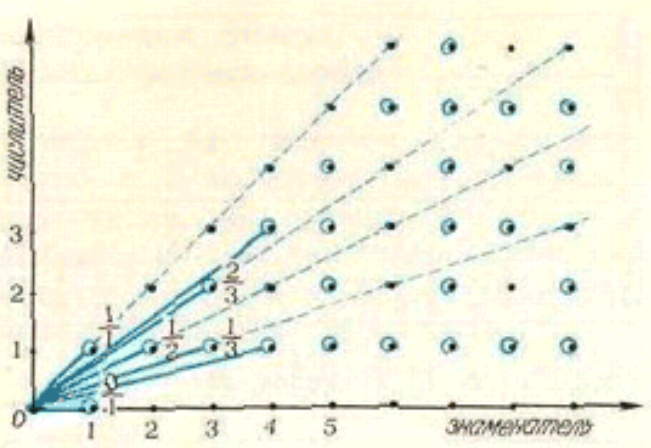
\includegraphics[width=8cm]{risunok.png}\\
\caption{Рис. 1}
\end{center}

Обратим внимание на знаменатели дробей в таблице 1. Составим для удобства из них новую таблицу 3. Правило $B$ позволяет продолжать "таблицу знаменателей" (не заботясь о числителях) следующим образом.
}
\end{multicols*}